\begin{aosachapter}{Web Spreadsheet}{s:spreadsheet}{Audrey Tang}

This chapter introduces a
\href{http://audreyt.github.io/500lines/spreadsheet/}{web spreadsheet}
written in
\href{https://github.com/audreyt/500lines/tree/master/spreadsheet/code}{99
lines} of the three languages natively supported by web browsers: HTML,
JavaScript, and CSS.

The ES5 version of this project is available as a
\href{http://jsfiddle.net/audreyt/LtDyP/}{jsFiddle}.

\aosasecti{Introduction}\label{introduction}

When Tim Berners-Lee invented the web in 1990, \emph{web pages} were
written in HTML by marking up text with angle-bracketed \emph{tags},
assigning a logical structure to the content. Text marked up within
\texttt{\textless{}a\textgreater{}\ldots{}\textless{}/a\textgreater{}}
became \emph{hyperlinks} that would refer the user to other pages on the
web.

In the 1990s, browsers added various presentational tags to the HTML
vocabulary, including some notoriously nonstandard tags such as
\texttt{\textless{}blink\textgreater{}\ldots{}\textless{}/blink\textgreater{}}
from Netscape Navigator and
\texttt{\textless{}marquee\textgreater{}\ldots{}\textless{}/marquee\textgreater{}}
from Internet Explorer, causing widespread problems in usability and
browser compatibility.

In order to restrict HTML to its original purpose---describing a
document's logical structure---browser makers eventually agreed to
support two additional languages: CSS to describe presentational styles
of a page, and JavaScript (JS) to describe its dynamic interactions.

Since then, the three languages have become more concise and powerful
through twenty years of co-evolution. In particular, improvements in JS
engines made it practical to deploy large-scale JS frameworks, such as
\href{http://angularjs.org/}{AngularJS}.

Today, cross-platform \emph{web applications} (such as web spreadsheets)
are as ubiquitous and popular as platform-specific applications (such as
VisiCalc, Lotus 1-2-3 and Excel) from the previous century.

How many features can a web application offer in 99 lines with
AngularJS? Let's see it in action!

\aosasecti{Overview}\label{overview}

The
\href{https://github.com/audreyt/500lines/tree/master/spreadsheet/code}{spreadsheet}
directory contains our showcase for late-2014 editions of the three web
languages: \href{http://www.w3.org/TR/html5/}{HTML5} for structure,
\href{http://www.w3.org/TR/css3-ui/}{CSS3} for presentation, and the JS
\href{http://git.io/es6features}{ES6 ``Harmony''} standard for
interaction. It also uses
\href{http://www.whatwg.org/specs/web-apps/current-work/multipage/webstorage.html}{web
storage} for data persistence and
\href{http://www.whatwg.org/specs/web-apps/current-work/multipage/workers.html}{web
workers} for running JS code in the background. As of this writing,
these web standards are supported by Firefox, Chrome, and Internet
Explorer 11+, as well as mobile browsers on iOS 5+ and Android 4+.

Now let's open \href{http://audreyt.github.io/500lines/spreadsheet/}{our
spreadsheet} in a browser (\aosafigref{500l.spreadsheet.initial}):

\aosafigure{spreadsheet-images/01-initial.png}{Initial Screen}{500l.spreadsheet.initial}

\aosasectii{Basic Concepts}\label{basic-concepts}

The spreadsheet spans two dimensions, with \emph{columns} starting from
\textbf{A}, and \emph{rows} starting from \textbf{1}. Each \emph{cell}
has a unique \emph{coordinate} (such as \textbf{A1}) and \emph{content}
(such as ``1874''), which belongs to one of four \emph{types}:

\begin{aosaitemize}

\item
  Text: ``+'' in \textbf{B1} and ``⇒'' in \textbf{D1}, aligned to the
  left.
\item
  Number: ``1874'' in \textbf{A1} and ``2046'' in \textbf{C1}, aligned
  to the right.
\item
  Formula: \texttt{=A1+C1} in \textbf{E1}, which \emph{calculates} to
  the \emph{value} ``3920'', displayed with a light blue background.
\item
  Empty: All cells in row \textbf{2} are currently empty.
\end{aosaitemize}

Click ``3920'' to set \emph{focus} on \textbf{E1}, revealing its formula
in an \emph{input box} (\aosafigref{500l.spreadsheet.inputbox}):

\aosafigure{spreadsheet-images/02-input.png}{Input Box}{500l.spreadsheet.input}

Now let's set focus on \textbf{A1} and \emph{change} its content to
``1'', causing \textbf{E1} to \emph{recalculate} its value to ``2047''
(\aosafigref{500l.spreadsheet.changed}):

\aosafigure{spreadsheet-images/03-changed.png}{Changed Content}{500l.spreadsheet.changed}

Press \textbf{ENTER} to set focus to \textbf{A2} and change its content
to \texttt{=Date()}, then press \textbf{TAB}, change the content of
\textbf{B2} to \texttt{=alert()}, then press \textbf{TAB} again to set
focus to \texttt{C2} (\aosafigref{500l.spreadsheet.error}):

\aosafigure{spreadsheet-images/04-error.png}{Formula Error}{500l.spreadsheet.error}

This shows that a formula may calculate to a number (``2047'' in
\textbf{E1}), a text (the current time in \textbf{A2}, aligned to the
left), or an \emph{error} (red letters in \textbf{B2}, aligned to the
center).

Next, let's try entering \texttt{=for(;;)\{\}}, the JS code for an
infinite loop that never terminates. The spreadsheet will prevent this
by automatically \emph{restoring} the content of \textbf{C2} after an
attempted change.

Now reload the page in the browser with \textbf{Ctrl-R} or
\textbf{Cmd-R} to verify that the spreadsheet content is
\emph{persistent}, staying the same across browser sessions. To
\emph{reset} the spreadsheet to its original contents, press the `curved
arrow' button on the top-left corner.

\aosasectii{Progressive Enhancement}\label{progressive-enhancement}

Before we dive into the 99 lines of code, it's worthwhile to disable JS
in the browser, reload the page, and note the differences
(\aosafigref{500l.spreadsheet.nojs}):

\begin{aosaitemize}

\item
  Instead of a large grid, only a 2x2 table remains onscreen, with a
  single content cell.
\item
  Row and column labels are replaced by \texttt{\{\{ row \}\}} and
  \texttt{\{\{ col \}\}}.
\item
  Pressing the reset button produces no effect.
\item
  Pressing \textbf{TAB} or clicking into the first line of content still
  reveals an editable input box.
\end{aosaitemize}

\aosafigure{spreadsheet-images/05-nojs.png}{With JavaScript Disabled}{500l.spreadsheet.nojs}

When we disable the dynamic interactions (JS), the content structure
(HTML) and the presentational styles (CSS) remain in effect. If a
website is useful with both JS and CSS disabled, we say it adheres to
the \emph{progressive enhancement} principle, making its content
accessible to the largest audience possible.

Because our spreadsheet is a web application with no server-side code,
we must rely on JS to provide the required logic. However, it does work
correctly when CSS is not fully supported, such as with screen readers
and text-mode browsers.

\aosafigure[240pt]{spreadsheet-images/06-nocss.png}{With CSS Disabled}{500l.spreadsheet.nocss}

As shown in \aosafigref{500l.spreadsheet.nocss}, if we enable JS in the
browser and disable CSS instead, the effects are:

\begin{aosaitemize}

\item
  All background and foreground colors are gone.
\item
  The input box and the cell value are both displayed, instead of just
  one at a time.
\item
  Otherwise, the application still works the same as the full version.
\end{aosaitemize}

\aosasecti{Code Walkthrough}\label{code-walkthrough}

\aosafigref{500l.spreadsheet.architecture} shows the links between HTML
and JS components:

\aosafigure{spreadsheet-images/00-architecture.png}{Architecture Diagram}{500l.spreadsheet.architecture}

In order to make sense of the diagram, let's go through the four source
code files, in the same sequence as the browser loads them:

\begin{aosaitemize}

\item
  \textbf{index.html}: 19 lines
\item
  \textbf{main.js}: 38 lines (excluding comments and blank lines)
\item
  \textbf{worker.js}: 30 lines (excluding comments and blank lines)
\item
  \textbf{styles.css}: 12 lines
\end{aosaitemize}

\aosasectii{HTML}\label{html}

The first line in \texttt{index.html} declares that it's written in
HTML5 (\texttt{\textless{}!DOCTYPE html\textgreater{}}) with the UTF-8
encoding:

\begin{verbatim}
<!DOCTYPE html><html><head><meta charset="UTF-8">
\end{verbatim}

Without the \texttt{charset} declaration, the browser may display the
reset button's Unicode symbol \texttt{↻} as \texttt{↻}, an example of
\emph{mojibake}: garbled text caused by decoding issues.

The next three lines are JS declarations, placed within the
\texttt{head} section as usual:

\begin{verbatim}
  <script src="lib/angular.js"></script>
  <script src="main.js"></script>
  <script>try{ angular.module('500lines') }catch(e){ location="es5/index.html" }</script>
\end{verbatim}

The \texttt{\textless{}script src="\ldots{}"\textgreater{}} tags load JS
resources from the same path as the HTML page. For example, if the
current URL is
\texttt{http://audreyt.github.io/500lines/spreadsheet/index.html}, then
\texttt{lib/angular.js} refers to
\texttt{http://audreyt.github.io/500lines/spreadsheet/lib/angular.js}.

The \texttt{try\{ angular.module('500lines') \}} line tests if
\texttt{main.js} is loaded correctly; if not, it tells the browser to
navigate to \texttt{es5/index.html} instead. This \emph{redirect-based
graceful degradation} technique ensures that for pre-2015 browsers with
no ES6 support, we can use the translated-to-ES5 versions of JS programs
as a fallback.

The next two lines load the CSS resource, close the \texttt{head}
section, and begin the \texttt{body} section containing the user-visible
part:

\begin{verbatim}
  <link href="styles.css" rel="stylesheet">
</head><body ng-app="500lines" ng-controller="Spreadsheet" ng-cloak>
\end{verbatim}

The \texttt{ng-app} and \texttt{ng-controller} attributes above tell
\href{http://angularjs.org/}{AngularJS} to call the \texttt{500lines}
module's \texttt{Spreadsheet} function, which would return a
\emph{model}: an object that provides \emph{bindings} on the document
\emph{view}. (The \texttt{ng-cloak} attribute hides the document from
display until the bindings are in place.)

As a concrete example, when the user clicks the
\texttt{\textless{}button\textgreater{}} defined in the next line, its
\texttt{ng-click} attribute will trigger and call \texttt{reset()} and
\texttt{calc()}, two named functions provided by the JS model:

\begin{verbatim}
  <table><tr>
    <th><button type="button" ng-click="reset(); calc()">↻</button></th>
\end{verbatim}

The next line uses \texttt{ng-repeat} to display the list of column
labels on the top row:

\begin{verbatim}
    <th ng-repeat="col in Cols">{{ col }}</th>
\end{verbatim}

For example, if the JS model defines \texttt{Cols} as
\texttt{{[}"A","B","C"{]}}, then there will be three heading cells
(\texttt{th}) labeled accordingly. The \texttt{\{\{ col \}\}} notation
tells AngularJS to \emph{interpolate} the expression, filling the
contents in each \texttt{th} with the current value of \texttt{col}.

Similarly, the next two lines go through values in \texttt{Rows} ---
\texttt{{[}1,2,3{]}} and so on --- creating a row for each one and
labeling the leftmost \texttt{th} cell with its number:

\begin{verbatim}
  </tr><tr ng-repeat="row in Rows">
    <th>{{ row }}</th>
\end{verbatim}

Because the \texttt{\textless{}tr ng-repeat\textgreater{}} tag is not
yet closed by \texttt{\textless{}/tr\textgreater{}} , the \texttt{row}
variable is still available for expressions. The next line creates a
data cell (\texttt{td}) in the current row and uses both \texttt{col}
and \texttt{row} variables in its \texttt{ng-class} attribute:

\begin{verbatim}
    <td ng-repeat="col in Cols" ng-class="{ formula: ('=' === sheet[col+row][0]) }">
\end{verbatim}

A few things are going on here. In HTML, the \texttt{class} attribute
describes a \emph{set of class names} that allow CSS to style them
differently. The \texttt{ng-class} here evaluates the expression
\texttt{('=' === sheet{[}col+row{]}{[}0{]})}; if it is true, then the
\texttt{\textless{}td\textgreater{}} gets \texttt{formula} as an
additional class, which gives the cell a light-blue background as
defined in line 8 of \textbf{styles.css} with the \texttt{.formula}
\emph{class selector}.

The expression above checks if the current cell is a formula by testing
if \texttt{=} is the initial character (\texttt{{[}0{]}}) of the string
in \texttt{sheet{[}col+row{]}}, where \texttt{sheet} is a JS model
object with coordinates (such as \texttt{"E1"}) as properties, and cell
contents (such as \texttt{"=A1+C1"}) as values. Note that because
\texttt{col} is a string and not a number, the \texttt{+} in
\texttt{col+row} means concatenation instead of addition.

Inside the \texttt{\textless{}td\textgreater{}}, we give the user an
input box to edit the cell content stored in
\texttt{sheet{[}col+row{]}}:

\begin{verbatim}
       <input id="{{ col+row }}" ng-model="sheet[col+row]" ng-change="calc()"
        ng-model-options="{ debounce: 200 }" ng-keydown="keydown( $event, col, row )">
\end{verbatim}

Here, the key attribute is \texttt{ng-model}, which enables a
\emph{two-way binding} between the JS model and the input box's editable
content. In practice, this means that whenever the user makes a change
in the input box, the JS model will update \texttt{sheet{[}col+row{]}}
to match the content, and trigger its \texttt{calc()} function to
recalculate values of all formula cells.

To avoid repeated calls to \texttt{calc()} when the user presses and
holds a key, \texttt{ng-model-options} limits the update rate to once
every 200 milliseconds.

The \texttt{id} attribute here is interpolated with the coordinate
\texttt{col+row}. The \texttt{id} attribute of a HTML element must be
different from the \texttt{id} of all other elements in the same
document. This ensures that the \texttt{\#A1} \emph{ID selector} refers
to a single element, instead of a set of elements like the class
selector \texttt{.formula}. When the user presses the
\textbf{UP}/\textbf{DOWN}/\textbf{ENTER} keys, the keyboard-navigation
logic in \texttt{keydown()} will use ID selectors to determine which
input box to focus on.

After the input box, we place a \texttt{\textless{}div\textgreater{}} to
display the calculated value of the current cell, represented in the JS
model by objects \texttt{errs} and \texttt{vals}:

\begin{verbatim}
      <div ng-class="{ error: errs[col+row], text: vals[col+row][0] }">
        {{ errs[col+row] || vals[col+row] }}</div>
\end{verbatim}

If an error occurs when computing a formula, the text interpolation uses
the error message contained in \texttt{errs{[}col+row{]}}, and
\texttt{ng-class} applies the \texttt{error} class to the element,
allowing CSS to style it differently (with red letters, aligned to the
center, etc.).

When there is no error, the \texttt{vals{[}col+row{]}} on the right side
of \texttt{\textbar{}\textbar{}} is interpolated instead. If it's a
non-empty string, the initial character (\texttt{{[}0{]}}) will evaluate
to true, applying the \texttt{text} class to the element that
left-aligns the text.

Because empty strings and numeric values have no initial character,
\texttt{ng-class} will not assign them any classes, so CSS can style
them with right alignment as the default case.

Finally, we close the \texttt{ng-repeat} loop in the column level with
\texttt{\textless{}/td\textgreater{}}, close the row-level loop with
\texttt{\textless{}/tr\textgreater{}}, and end the HTML document with:

\begin{verbatim}
    </td>
  </tr></table>
</body></html>
\end{verbatim}

\aosasectii{JS: Main Controller}\label{js-main-controller}

The \texttt{main.js} file defines the \texttt{500lines} module and its
\texttt{Spreadsheet} controller function, as required by the
\texttt{\textless{}body\textgreater{}} element in \texttt{index.html}.

As the bridge between the HTML view and the background worker, it has
four tasks:

\begin{aosaitemize}

\item
  Define the dimensions and labels of columns and rows.
\item
  Provide event handlers for keyboard navigation and the reset button.
\item
  When the user changes the spreadsheet, send its new content to the
  worker.
\item
  When computed results arrive from the worker, update the view and save
  the current state.
\end{aosaitemize}

The flowchart below shows the controller-worker interaction in more
detail:

\begin{figure}[htbp]
\centering
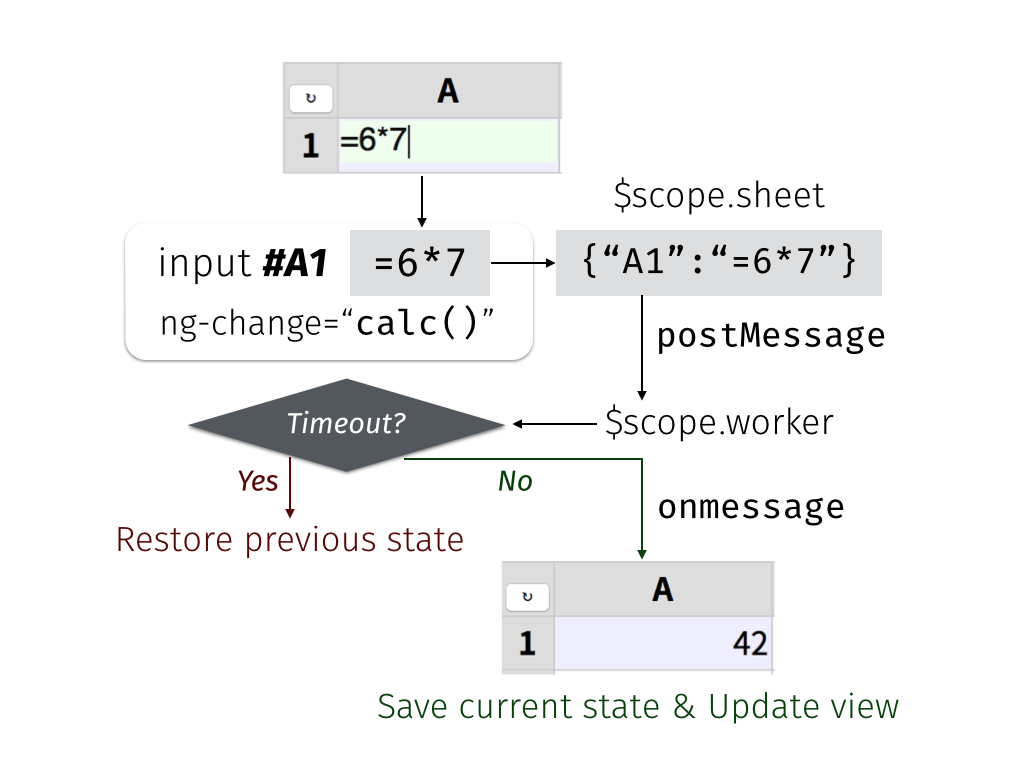
\includegraphics{./images/00-flowchart.png}
\caption{Controller-Worker Flowchart}
\end{figure}

Now let's walk through the code. In the first line, we request the JS
model \texttt{\$scope} object from AngularJS:

\begin{verbatim}
angular.module('500lines', []).controller('Spreadsheet', function ($scope, $timeout) {
\end{verbatim}

The \texttt{\$} in \texttt{\$scope} is part of the variable name. Here
we also request the
\href{https://docs.angularjs.org/api/ng/service/\$timeout}{\texttt{\$timeout}}
service function from AngularJS; later on, we will use it to prevent
infinite-looping formulas.

To put \texttt{Cols} and \texttt{Rows} into the model, simply define
them as properties of \texttt{\$scope}:

\begin{verbatim}
  // Begin of $scope properties; start with the column/row labels
  $scope.Cols = [], $scope.Rows = [];
  for (col of range( 'A', 'H' )) { $scope.Cols.push(col); }
  for (row of range( 1, 20 )) { $scope.Rows.push(row); }
\end{verbatim}

The ES6
\href{https://developer.mozilla.org/en-US/docs/Web/JavaScript/Reference/Statements/for...of}{for\ldots{}of}
syntax makes it easy to loop through ranges with a start and an end
point, with the helper function \texttt{range} defined as a
\href{https://developer.mozilla.org/en-US/docs/Web/JavaScript/Reference/Statements/function*}{generator}:

\begin{verbatim}
  function* range(cur, end) { while (cur <= end) { yield cur;
\end{verbatim}

The \texttt{function*} above means that \texttt{range} returns an
\href{https://developer.mozilla.org/en-US/docs/Web/JavaScript/Guide/The_Iterator_protocol}{iterator},
with a \texttt{while} loop that would
\href{https://developer.mozilla.org/en-US/docs/Web/JavaScript/Reference/Operators/yield}{\texttt{yield}}
a single value at a time. Whenever the \texttt{for} loop demands the
next value, it will resume execution right after the \texttt{yield}
line:

\begin{verbatim}
    // If it’s a number, increase it by one; otherwise move to next letter
    cur = (isNaN( cur ) ? String.fromCodePoint( cur.codePointAt()+1 ) : cur+1);
  } }
\end{verbatim}

To generate the next value, we use \texttt{isNaN} to see if \texttt{cur}
is meant as a letter (\texttt{NaN} stands for ``not a number.'') If so,
we get the letter's
\href{https://developer.mozilla.org/en-US/docs/Web/JavaScript/Reference/Global_Objects/String/codePointAt}{code
point value}, increment it by one, and
\href{https://developer.mozilla.org/en-US/docs/Web/JavaScript/Reference/Global_Objects/String/fromCodePoint}{convert
the codepoint} back to get its next letter. Otherwise, we simply
increase the number by one.

Next up, we define the \texttt{keydown()} function that handles keyboard
navigation across rows:

\begin{verbatim}
  // UP(38) and DOWN(40)/ENTER(13) move focus to the row above (-1) and below (+1).
  $scope.keydown = ({which}, col, row)=>{ switch (which) {
\end{verbatim}

The
\href{https://developer.mozilla.org/en-US/docs/Web/JavaScript/Reference/arrow_functions}{arrow
function} receives the arguments \texttt{(\$event, col, row)} from
\texttt{\textless{}input ng-keydown\textgreater{}}, using
\href{https://developer.mozilla.org/en-US/docs/Web/JavaScript/New_in_JavaScript/1.7\#Pulling_fields_from_objects_passed_as_function_parameter}{destructuring
assignment} to assign \texttt{\$event.which} into the \texttt{which}
parameter, and checks if it's among the three navigational key codes:

\begin{verbatim}
    case 38: case 40: case 13: $timeout( ()=>{
\end{verbatim}

If it is, we use \texttt{\$timeout} to schedule a change of cell focus
after the current \texttt{ng-keydown} and \texttt{ng-change} handler.
Because \texttt{\$timeout} requires a function as argument, the
\texttt{()=\textgreater{}\{\ldots{}\}} syntax constructs a function to
represent the focus-change logic, which starts by checking the direction
of movement:

\begin{verbatim}
      const direction = (which === 38) ? -1 : +1;
\end{verbatim}

The \texttt{const} declarator means \texttt{direction} will not change
during the function's execution. The direction to move is either upward
(\texttt{-1}, from \textbf{A2} to \textbf{A1}) if the key code is 38
(\textbf{UP}), or downward (\texttt{+1}, from \textbf{A2} to
\textbf{A3}) otherwise.

Next up, we retrieve the target element using the ID selector syntax
(e.g. \texttt{"\#A3"}), constructed with a
\href{https://developer.mozilla.org/en-US/docs/Web/JavaScript/Reference/template_strings}{template
string} written in a pair of backticks, concatenating the leading
\texttt{\#}, the current \texttt{col} and the target
\texttt{row + direction}:

\begin{verbatim}
      const cell = document.querySelector( `#${ col }${ row + direction }` );
      if (cell) { cell.focus(); }
    } );
  } };
\end{verbatim}

We put an extra check on the result of \texttt{querySelector} because
moving upward from \textbf{A1} will produce the selector \texttt{\#A0},
which has no corresponding element, and so will not trigger a focus
change --- the same goes for pressing \textbf{DOWN} at the bottom row.

Next, we define the \texttt{reset()} function so the \texttt{↻} button
can restore the initial contents of the \texttt{sheet}:

\begin{verbatim}
  // Default sheet content, with some data cells and one formula cell.
  $scope.reset = ()=>{ $scope.sheet = { A1: 1874, B1: '+', C1: 2046, D1: '⇒', E1: '=A1+C1' }; }
\end{verbatim}

The \texttt{init()} function tries restoring the \texttt{sheet} content
from its previous state from the
\href{https://developer.mozilla.org/en-US/docs/Web/Guide/API/DOM/Storage\#localStorage}{localStorage},
and defaults to the initial content if it's our first time running the
application:

\begin{verbatim}
  // Define the initializer, and immediately call it
  ($scope.init = ()=>{
    // Restore the previous .sheet; reset to default if it’s the first run
    $scope.sheet = angular.fromJson( localStorage.getItem( '' ) );
    if (!$scope.sheet) { $scope.reset(); }
    $scope.worker = new Worker( 'worker.js' );
  }).call();
\end{verbatim}

A few things are worth nothing in the \texttt{init()} function above:

\begin{aosaitemize}

\item
  We use the
  \texttt{(\$scope.init = ()=\textgreater{}\{\ldots{}\}).call()} syntax
  to define the function and immediately call it.
\item
  Because localStorage only stores strings, we \emph{parse} the
  \texttt{sheet} structure from its
  \href{https://developer.mozilla.org/en-US/docs/Glossary/JSON}{JSON}
  representation using \texttt{angular.fromJson()}.
\item
  At the last step of \texttt{init()}, we create a new
  \href{https://developer.mozilla.org/en-US/docs/Web/API/Worker}{web
  worker} thread and assign it to the \texttt{worker} scope property.
  Although the worker is not directly used in the view, it's customary
  to use \texttt{\$scope} to share objects used across model functions,
  in this case between \texttt{init()} here and \texttt{calc()} below.
\end{aosaitemize}

While \texttt{sheet} holds the user-editable cell content, \texttt{errs}
and \texttt{vals} contain the results of calculations --- errors and
values --- that are read-only to the user:

\begin{verbatim}
  // Formula cells may produce errors in .errs; normal cell contents are in .vals
  [$scope.errs, $scope.vals] = [ {}, {} ];
\end{verbatim}

With these properties in place, we can define the \texttt{calc()}
function that triggers whenever the user makes a change to
\texttt{sheet}:

\begin{verbatim}
  // Define the calculation handler; not calling it yet
  $scope.calc = ()=>{
    const json = angular.toJson( $scope.sheet );
\end{verbatim}

Here we first take a snapshot of the state of \texttt{sheet} and store
it in the constant \texttt{json}, a JSON string.

Next up, we construct a \texttt{promise} from
\href{https://docs.angularjs.org/api/ng/service/\$timeout}{\$timeout}
that cancels the upcoming computation if it takes more than 99
milliseconds:

\begin{verbatim}
    const promise = $timeout( ()=>{
      // If the worker has not returned in 99 milliseconds, terminate it
      $scope.worker.terminate();
      // Back up to the previous state and make a new worker
      $scope.init();
      // Redo the calculation using the last-known state
      $scope.calc();
    }, 99 );
\end{verbatim}

Since we made sure that \texttt{calc()} is called at most once every 200
milliseconds via the
\texttt{\textless{}input ng-model-options\textgreater{}} attribute in
HTML, this arrangement leaves 101 milliseconds for \texttt{init()} to
restore \texttt{sheet} to the last known-good state and make a new
worker.

The worker's task is to calculate \texttt{errs} and \texttt{vals} from
the contents of\texttt{sheet}. Because \textbf{main.js} and
\textbf{worker.js} communicate by message-passing, we need an
\texttt{onmessage} handler to receive the results once they are ready:

\begin{verbatim}
    // When the worker returns, apply its effect on the scope
    $scope.worker.onmessage = ({data})=>{
      $timeout.cancel( promise );
      localStorage.setItem( '', json );
      $timeout( ()=>{ [$scope.errs, $scope.vals] = data; } );
    };
\end{verbatim}

If \texttt{onmessage} is called, we know that the \texttt{sheet}
snapshot in \texttt{json} is stable (i.e., containing no
infinite-looping formulas), so we cancel the 99-millisecond timeout,
write the snapshot to localStorage, and schedule a UI update with a
\texttt{\$timeout} function that updates \texttt{errs} and \texttt{vals}
to the user-visible view.

With the handler in place, we can post the state of \texttt{sheet} to
the worker, starting its calculation in the background:

\begin{verbatim}
    // Post the current sheet content for the worker to process
    $scope.worker.postMessage( $scope.sheet );
  };

  // Start calculation when worker is ready
  $scope.worker.onmessage = $scope.calc;
  $scope.worker.postMessage( null );
});
\end{verbatim}

\aosasectii{JS: Background Worker}\label{js-background-worker}

There are three reasons for using a web worker to calculate formulas,
instead of using the main JS thread for the task:

\begin{aosaitemize}

\item
  While the worker runs in the background, the user is free to continue
  interacting with the spreadsheet without getting blocked by
  computation in the main thread.
\item
  Because we accept any JS expression in a formula, the worker provides
  a \emph{sandbox} that prevents formulas from interfering with the page
  that contains them, such as by popping out an \texttt{alert()} dialog.
\item
  A formula can refer to any coordinates as variables. The other
  coordinates may contain another formula that might end in a cyclic
  reference. To solve this problem, we use the worker's \emph{global
  scope} object \texttt{self}, and define these variables as
  \emph{getter functions} on \texttt{self} to implement the
  cycle-prevention logic.
\end{aosaitemize}

With these in mind, let's take a look at the worker's code.

The worker's sole purpose is defining its \texttt{onmessage} handler.
The handler takes \texttt{sheet}, calculates \texttt{errs} and
\texttt{vals}, and posts them back to the main JS thread. We begin by
re-initializing the three variables when we receive a message:

\begin{verbatim}
let sheet, errs, vals;
self.onmessage = ({data})=>{
  [sheet, errs, vals] = [ data, {}, {} ];
\end{verbatim}

In order to turn coordinates into global variables, we first iterate
over each property in \texttt{sheet}, using a \texttt{for\ldots{}in}
loop:

\begin{verbatim}
  for (const coord in sheet) {
\end{verbatim}

ES6 introduces \texttt{const} and \texttt{let} declares \emph{block
scoped} constants and variables; \texttt{const coord} above means that
functions defined in the loop would capture the specific value of
\texttt{coord} in each iteration.

In contrast, \texttt{var coord} in earlier versions of JS would declare
a \emph{function scoped} variable, and functions defined in each loop
iteration would end up pointing to the same \texttt{coord} variable.

Customarily, formula variables are case-insensitive and can optionally
have a \texttt{\$} prefix. Because JS variables are case-sensitive, we
use two \texttt{map} calls to go over the four variable names for the
same coordinate:

\begin{verbatim}
    // Four variable names pointing to the same coordinate: A1, a1, $A1, $a1
    [ '', '$' ].map( p => [ coord, coord.toLowerCase() ].map(c => {
      const name = p+c;
\end{verbatim}

Note the shorthand arrow function syntax above:
\texttt{p =\textgreater{} ...} is the same as
\texttt{(p) =\textgreater{} \{ ... \}}.

For each variable name, like \texttt{A1} and \texttt{\$a1}, we define an
\href{https://developer.mozilla.org/en-US/docs/Web/JavaScript/Reference/Global_Objects/Object/defineProperty}{accessor
property} on \texttt{self} that calculates \texttt{vals{[}"A1"{]}}
whenever they are evaluated in an expression:

\begin{verbatim}
      // Worker is reused across calculations, so only define each variable once
      if ((Object.getOwnPropertyDescriptor( self, name ) || {}).get) { return; }

      // Define self['A1'], which is the same thing as the global variable A1
      Object.defineProperty( self, name, { get() {
\end{verbatim}

The \texttt{\{ get() \{ \ldots{} \} \}} syntax above is shorthand for
\texttt{\{ get: ()=\textgreater{}\{ \ldots{} \} \}}. Because we define
only \texttt{get} and not \texttt{set}, the variables become
\emph{read-only} and cannot be modified from user-supplied formulas.

The \texttt{get} accessor starts by checking \texttt{vals{[}coord{]}},
and simply returns it if it's already calculated:

\begin{verbatim}
        if (coord in vals) { return vals[coord]; }
\end{verbatim}

If not, we need to calculate \texttt{vals{[}coord{]}} from
\texttt{sheet{[}coord{]}}.

First we set it to \texttt{NaN}, so self-references like setting
\textbf{A1} to \texttt{=A1} will end up with \texttt{NaN} instead of an
infinite loop:

\begin{verbatim}
        vals[coord] = NaN;
\end{verbatim}

Next we check if \texttt{sheet{[}coord{]}} is a number by converting it
to numeric with prefix \texttt{+}, assigning the number to \texttt{x},
and comparing its string representation with the original string. If
they differ, then we set \texttt{x} to the original string:

\begin{verbatim}
        // Turn numeric strings into numbers, so =A1+C1 works when both are numbers
        let x = +sheet[coord];
        if (sheet[coord] !== x.toString()) { x = sheet[coord]; }
\end{verbatim}

If the initial character of \texttt{x} is \texttt{=}, then it's a
formula cell. We evaluate the part after \texttt{=} with
\texttt{eval.call()}, using the first argument \texttt{null} to tell
\texttt{eval} to run in the \emph{global scope}, hiding the
\emph{lexical scope} variables like \texttt{x} and \texttt{sheet} from
the evaluation:

\begin{verbatim}
        // Evaluate formula cells that begin with =
        try { vals[coord] = (('=' === x[0]) ? eval.call( null, x.slice( 1 ) ) : x);
\end{verbatim}

If the evaluation succeeds, the result is stored into
\texttt{vals{[}coord{]}}. For non-formula cells, the value of
\texttt{vals{[}coord{]}} is simply \texttt{x}, which may be a number or
a string.

If \texttt{eval} results in an error, the \texttt{catch} block tests if
it's because the formula refers to an empty cell not yet defined in
\texttt{self}:

\begin{verbatim}
        } catch (e) {
          const match = /\$?[A-Za-z]+[1-9][0-9]*\b/.exec( e );
          if (match && !( match[0] in self )) {
\end{verbatim}

In that case, we set the missing cell's default value to ``0'', clear
\texttt{vals{[}coord{]}}, and re-run the current computation using
\texttt{self{[}coord{]}}:

\begin{verbatim}
            // The formula refers to a uninitialized cell; set it to 0 and retry
            self[match[0]] = 0;
            delete vals[coord];
            return self[coord];
          }
\end{verbatim}

If the user gives the missing cell a content later on in
\texttt{sheet{[}coord{]}}, then \texttt{Object.defineProperty} would
take over and override the temporary value.

Other kinds of errors are stored in \texttt{errs{[}coord{]}}:

\begin{verbatim}
          // Otherwise, stringify the caught exception in the errs object
          errs[coord] = e.toString();
        }
\end{verbatim}

In case of errors, the value of \texttt{vals{[}coord{]}} will remain
\texttt{NaN} because the assignment did not complete.

Finally, the \texttt{get} accessor returns the calculated value stored
in \texttt{vals{[}coord{]}}, which must be a number, a Boolean value, or
a string:

\begin{verbatim}
        // Turn vals[coord] into a string if it's not a number or Boolean
        switch (typeof vals[coord]) { case 'function': case 'object': vals[coord]+=''; }
        return vals[coord];
      } } );
    }));
  }
\end{verbatim}

With accessors defined for all coordinates, the worker goes through the
coordinates again, invoking each accessor with \texttt{self{[}coord{]}},
then posts the resulting \texttt{errs} and \texttt{vals} back to the
main JS thread:

\begin{verbatim}
  // For each coordinate in the sheet, call the property getter defined above
  for (const coord in sheet) { self[coord]; }
  return [ errs, vals ];
}
\end{verbatim}

\aosasectii{CSS}\label{css}

The \textbf{styles.css} file contains just a few selectors and their
presentational styles. First, we style the table to merge all cell
borders together, leaving no spaces between neighboring cells:

\begin{verbatim}
table { border-collapse: collapse; }
\end{verbatim}

Both the heading and data cells share the same border style, but we can
tell them apart by their background colors: heading cells are light
gray, data cells are white by default, and formula cells get a light
blue background:

\begin{verbatim}
th, td { border: 1px solid #ccc; }
th { background: #ddd; }
td.formula { background: #eef; }
\end{verbatim}

The displayed width is fixed for each cell's calculated values. Empty
cells receive a minimal height, and long lines are clipped with a
trailing ellipsis:

\begin{verbatim}
td div { text-align: right; width: 120px; min-height: 1.2em;
         overflow: hidden; text-overflow: ellipsis; }
\end{verbatim}

The text alignment and decorations are determined by each value's type,
as reflected by the \texttt{text} and \texttt{error} class selectors:

\begin{verbatim}
div.text { text-align: left; }
div.error { text-align: center; color: #800; font-size: 90%; border: solid 1px #800 }
\end{verbatim}

As for the user-editable \texttt{input} box, we use \emph{absolute
positioning} to overlay it on top of its cell, and make it transparent
so the underlying \texttt{div} with the cell's value shows through:

\begin{verbatim}
input { position: absolute; border: 0; padding: 0;
        width: 120px; height: 1.3em; font-size: 100%;
        color: transparent; background: transparent; }
\end{verbatim}

When the user sets focus on the input box, it springs into the
foreground:

\begin{verbatim}
input:focus { color: #111; background: #efe; }
\end{verbatim}

Furthermore, the underlying \texttt{div} is collapsed into a single
line, so it's completely covered by the input box:

\begin{verbatim}
input:focus + div { white-space: nowrap; }
\end{verbatim}

\aosasecti{Conclusion}\label{conclusion}

Since this book is \emph{500 Lines or Less}, a web spreadsheet in 99
lines is a minimal example --- please feel free to experiment and extend
it in any direction you'd like.

Here are some ideas, all easily reachable in the remaining space of 401
lines:

\begin{aosaitemize}

\item
  A collaborative online editor using
  \href{http://sharejs.org/}{ShareJS},
  \href{http://angularfire.com}{AngularFire} or
  \href{http://goangular.org/}{GoAngular}.
\item
  Markdown syntax support for text cells, using
  \href{http://ngmodules.org/modules/angular-marked}{angular-marked}.
\item
  Common formula functions (\texttt{SUM}, \texttt{TRIM}, etc.) from the
  \href{https://en.wikipedia.org/wiki/OpenFormula}{OpenFormula
  standard}.
\item
  Interoperate with popular spreadsheet formats, such as CSV and
  SpreadsheetML via \href{http://sheetjs.com/}{SheetJS}.
\item
  Import from and export to online spreadsheet services, such as Google
  Spreadsheet and \href{http://ethercalc.net/}{EtherCalc}.
\end{aosaitemize}

\aosasectii{A Note on JS versions}\label{a-note-on-js-versions}

This chapter aims to demonstrate new concepts in ES6, so we use the
\href{https://github.com/google/traceur-compiler}{Traceur compiler} to
translate source code to ES5 to run on pre-2015 browsers.

If you prefer to work directly with the 2010 edition of JS, the
\href{https://audreyt.github.io/500lines/spreadsheet/as-javascript-1.8.5/}{as-javascript-1.8.5}
directory has \textbf{main.js} and \textbf{worker.js} written in the
style of ES5; the
\href{https://github.com/audreyt/500lines/tree/master/spreadsheet/as-javascript-1.8.5}{source
code} is line-by-line comparable to the ES6 version with the same line
count.

For people preferring a cleaner syntax, the
\href{https://audreyt.github.io/500lines/spreadsheet/as-livescript-1.3.0/}{as-livescript-1.3.0}
directory uses \href{http://livescript.net/}{LiveScript} instead of ES6
to write \textbf{main.ls} and \textbf{worker.ls}; the
\href{https://github.com/audreyt/500lines/tree/master/spreadsheet/as-livescript-1.3.0}{source
code} is 20 lines shorter than the JS version.

Building on the LiveScript language, the
\href{https://audreyt.github.io/500lines/spreadsheet/as-react-livescript/}{as-react-livescript}
directory uses the \href{https://facebook.github.io/react/}{ReactJS}
framework; the
\href{https://github.com/audreyt/500lines/tree/master/spreadsheet/as-react-livescript}{source
code} is 10 lines more than the AngularJS equivalent, but runs
considerably faster.

If you are interested in translating this example to alternate JS
languages, send a \href{https://github.com/audreyt/500lines/pulls}{pull
request} --- I'd love to hear about it!

\end{aosachapter}
